\section{Introduction}

There are works on helping people read \cite{keshav2007read} and write \cite{hall2008write, zobel2004writing} papers (formally documented literature).
I was just looking for the ideal LaTeX configuration I would love to write (and read) in, and I could not find one; so I made one (and you're now reading it). Feel free to use this template if you like it. Obviously, I absolve myself from all liabilities. This is not targeted for any particular conference, workshop, or anything. The ideal purpose is to serve as a multi-contributor backbone, with suggestions and everything. 

Ignore all the \textsc{Lorem ipsum}. I try my best to use it only as a placeholder to fill up space. I do put useful things in the source of \LaTeX, so keep an eye out for them.

% Figure in the middle of text, but display at top (after abstract barrier)
%   Should be single column
\begin{figure}[t]
    \centering
    % Anything less than 50% will be in one column
    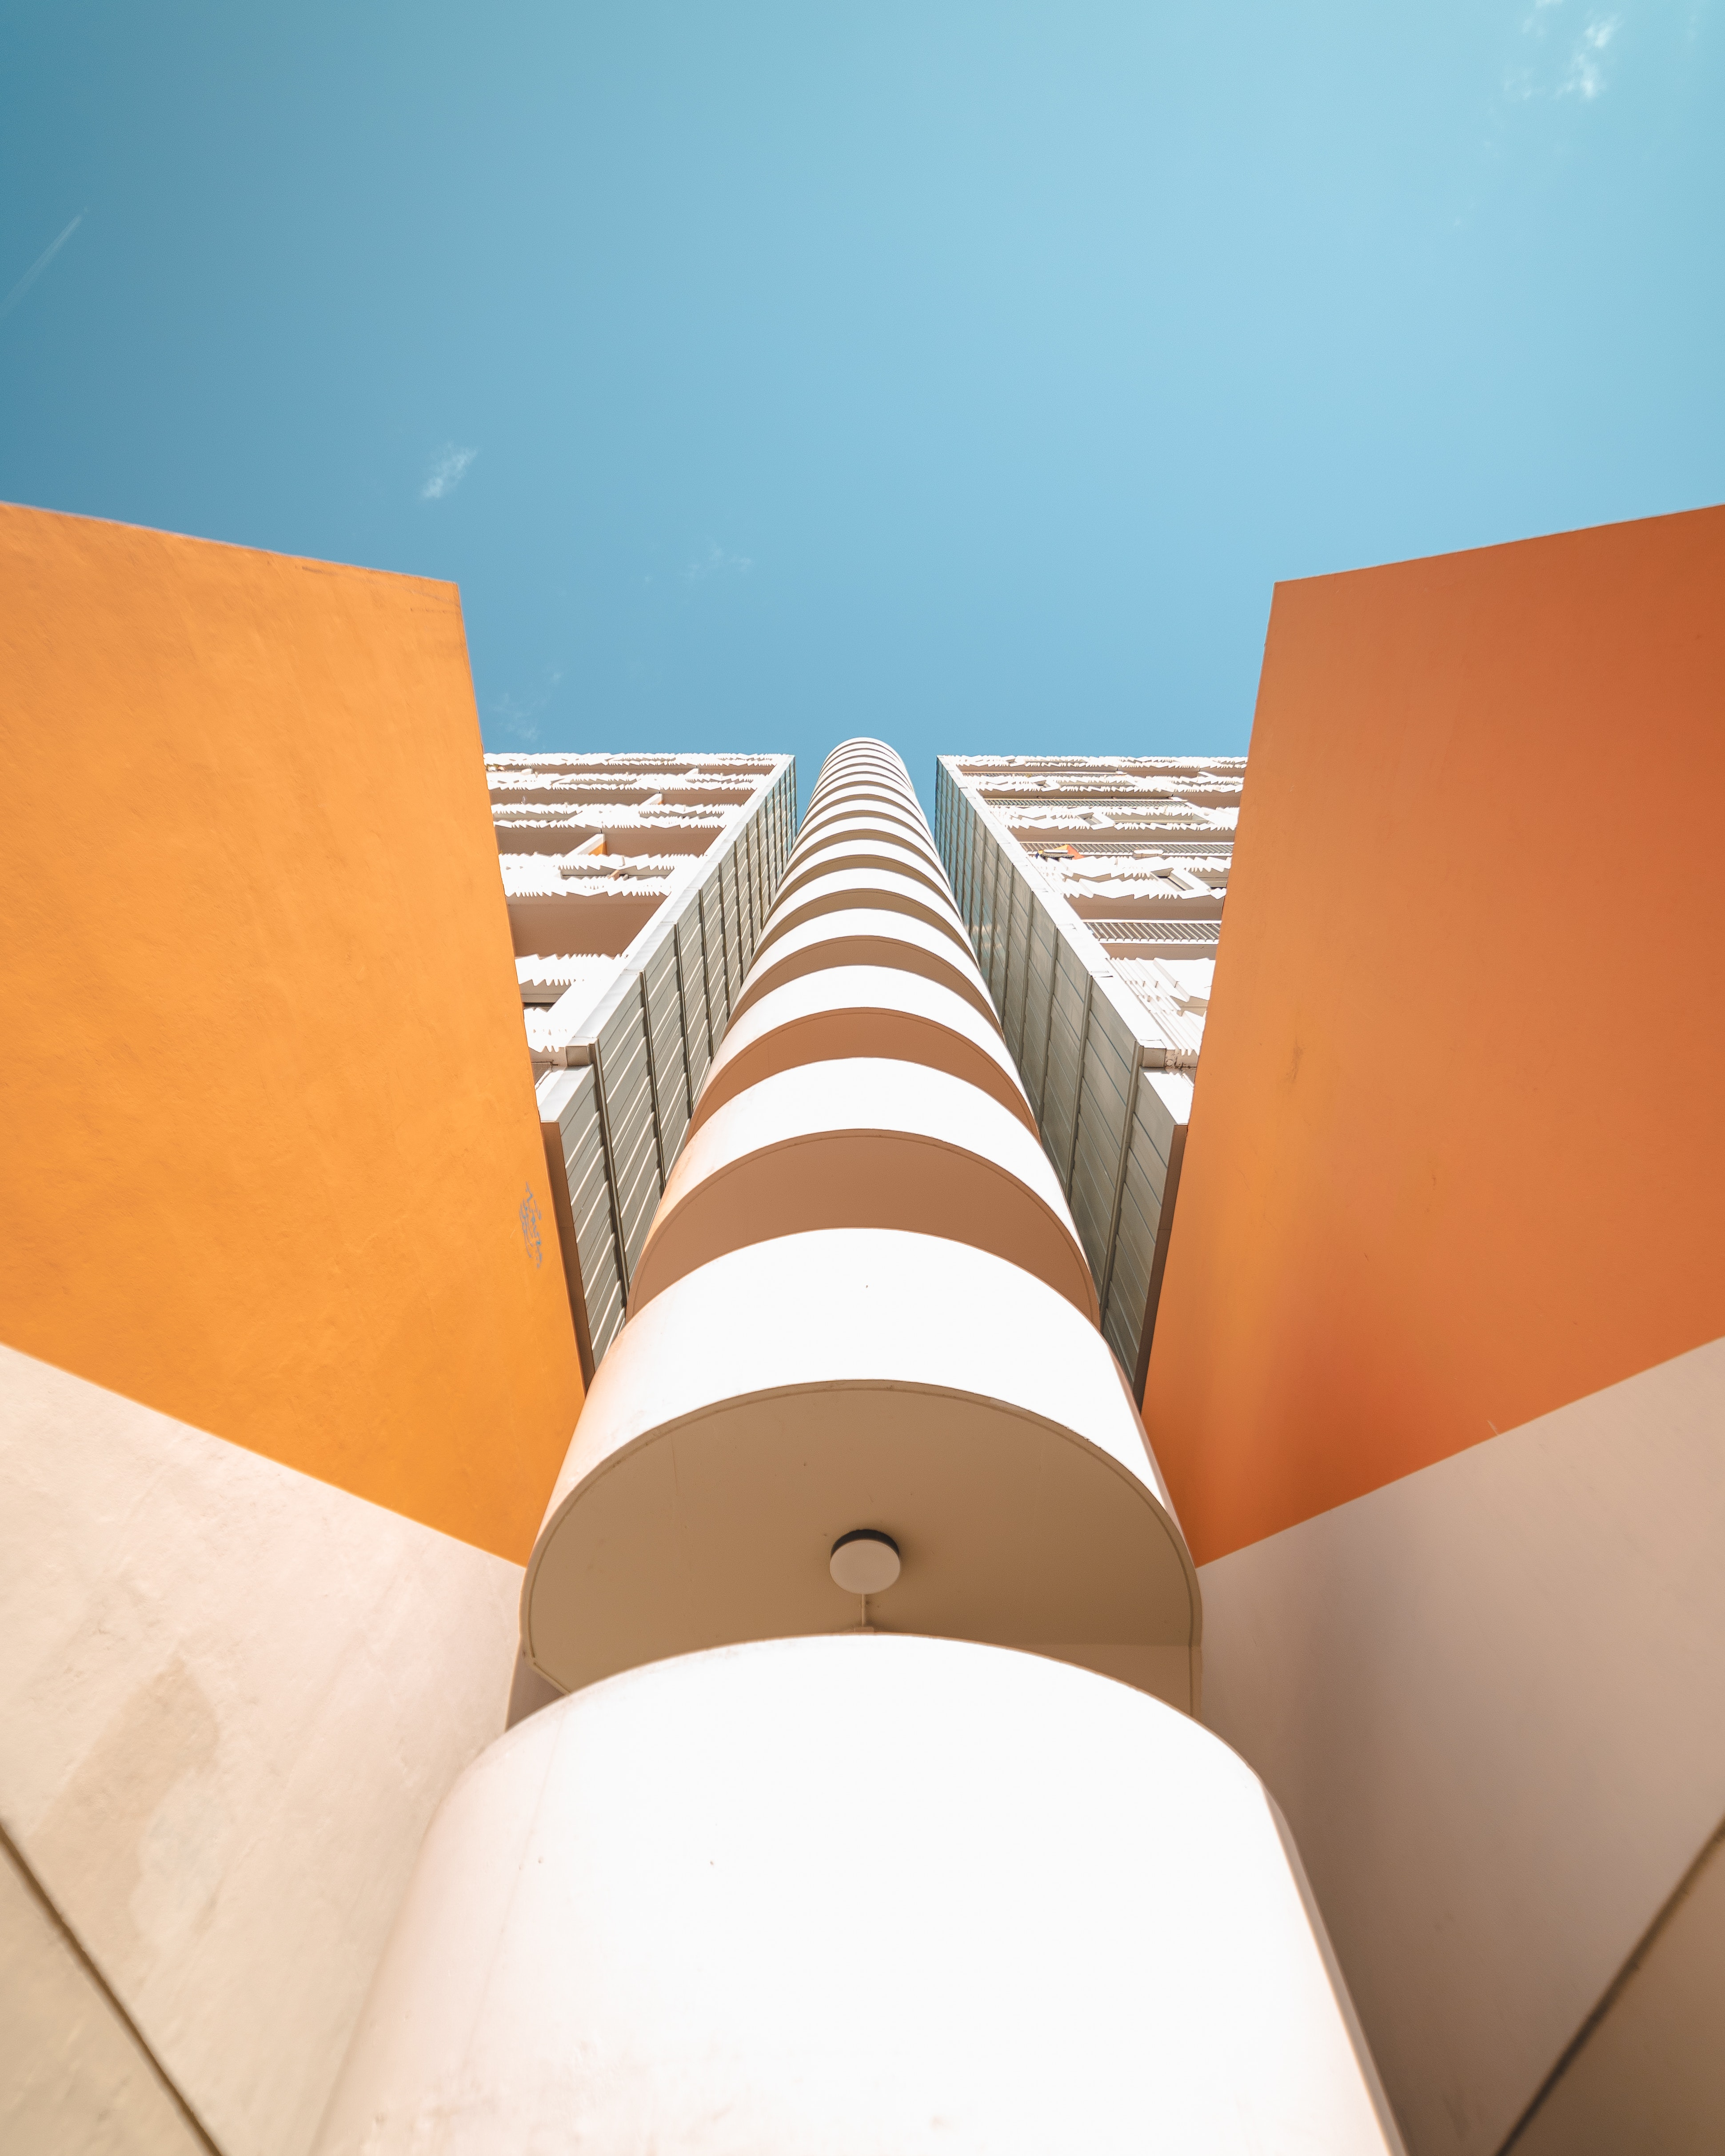
\includegraphics[width=0.45 \textwidth]{building1.jpg}
    \caption{A simple building figure}
    \label{fig:building}
    \small
        This figure serves as a top \emph{teaser} figure in most papers. This particular one is \href{https://www.pexels.com/photo/high-rise-orange-and-white-building-2739074/}{Photo by Guillaume Meurice from Pexels}
\end{figure}

\lipsum[1]

The \emph{contributions} of this work are as follows

\begin{enumerate}
    \item A useful template for myself, bringing together many concepts of \LaTeX;
    \item A guide to using the \href{https://www.ctan.org/pkg/coop-writing}{coop-writing} package to emulate multi-author settings;
    \item Emulate a workflow of an actual paper
    \begin{itemize}
        \item A paper with most of the conventional items like images, equations, tables, etc.
        \item This paper also has a teaser figure~\ref{fig:building}.
    \end{itemize}
    \item Just to increase the amount of work available in the world of \LaTeX. Maybe to give something back to the community.
\end{enumerate}
